\subsection{The Halved Model}
\label{sec:add.add.halved}

The idea behind the halved model is that the archetypal model can be looked at differently, because it is a circle map.
Let $m$ be the archetypal model for this section.
We know the model $m$ maps an input $x$ to $f(x) \mod 1$, meaning that if the output $f(x)$ is greater or equal to 1 we subtract 1 from it until it is in the range $[0, 1)$.
Similarly, we add 1 to it if it is smaller than 0 until it is in the desired range.
Now instead of confining the model to the domain of $[0, 1)$, we think of it repeating infinitely in both directions.
This process is called lifting of circle maps and is described by \Citeauthor{devaney2021introduction} in his book~\cite{devaney2021introduction}.
We can achieve this by mapping $T^m: x \mapsto f(x - \lfloor x \rfloor)$.
This trick maps any input $x \in \mathbb{R}$ into the domain $[0, 1)$ of the archetypal model $m$ and causes $T^m$ to repeat infinitely.
$T^m$ is now a lift of the model $m$ in the domain of all real numbers $\mathbb{R}$.
\Cref{fig:add.halved.lift} illustrates this concept for the cycle in the parameter region $P^{14}_3$.
The blue square is the full model.
One can see, that the branch $f_\D$ is outside the blue square at its right edge.
This is because it was cut off and continued at the bottom of the square before, due to the $\mod 1$ operation.

\begin{figure}
	\centering
	\includegraphics[width=.7 \textwidth]{63_MinimalRepr_Adding_Halved/Cob_Vis_s/Manual/result.png}
	\caption{Illustration of the lifted archetypal model}
	\label{fig:add.halved.lift}
\end{figure}

In this model, there are no cycles that have multiple rotations.
Instead, the cycles that had multiple rotations in the full model, manifest as a sequence of different blocks of the full model.
Meaning for the example $P^{14}_3$, the same blocks of $\A^4\B^3\C^4\D^3$ are repeating infinitely.
But for an example with multiple rotations, such as $\A\B\C\D\A^2\B^2\C^2\D^2$, the blocks will not all be the same.
Instead, the blocks $\A\B\C\D$ and $\A^2\B^2\C^2\D^2$ will be alternating.

Now we will take advantage of the symmetry in the model function $f$ of the archetypal model.
Since $f(x + \frac{1}{2}) \equiv f(x) + \frac{1}{2} \mod 1$, we can split the lifted model $T^m$ into smaller blocks of size $\frac{1}{2}$.
The function of the infinite model repeats in these smaller blocks.
These blocks are marked red in \Cref{fig:add.halved.lift}.
The red blocks represent the halved model, it is the smallest repeating part of the lifted model $T^m$.
Basically we choose the smallest model, of which $T^m$ is a lift.
This happens to be exactly our model $m$ folded in half.
So the halved archetypal model maps $x \mapsto g(x) \mod \frac{1}{2}$, where $g(x)$ is the same as in the archetypal model defined in \Cref{sec:setup.arch.definition}.

When we scan the same area in the halved archetypal model as we did in \Cref{fig:add.add.like.hor.2D} for the horizontal \gls{pal} structures, we get one big structure that looks like \gls{pa}.
This is shown in \Cref{fig:add.halved.hor.2D}.
The red arrow indicates the parameter range for the 1D period scan in \Cref{fig:add.halved.hor.1D}.
The 1D scan shows that the periods in this structure add up as we would expect in \gls{pa} structures.

\begin{figure}
	\centering
	\subfloat[2D period scan]{
		\includegraphics[width=.45 \textwidth]{63_MinimalRepr_Adding_Halved/2D_Period_add_zoom_hor/result.png}
		\label{fig:add.halved.hor.2D}
	}
	\subfloat[1D period scan]{
		\includegraphics[width=.45 \textwidth]{63_MinimalRepr_Adding_Halved/1D_Period_hor_low/result.png}
		\label{fig:add.halved.hor.1D}
	}
	\caption[2D and 1D period scans of a horizontal period-adding structure in the halved increasing archetypal model]{
		2D and 1D period scans of a horizontal \gls{pa} structure in the halved increasing archetypal model.
		The fixed parameters are $a_L = 1, b_L = 0.8,$ and $g_R\left(\frac{1}{2}\right) = \frac{1}{2} + \frac{1}{40}$.
		(a) shows the 2D period scan where the parameters $\alpha = g_R\left(\frac{1}{4}\right)$ and $\beta = c_L$ are varied.
		The small arrow indicates the parameter range for the 1D period scan in (b).
		Here, only $\beta$ is varied.
		The numbers at the top mark the periods at the corresponding value for $\beta$.
	}
	\label{fig:add.halved.hor}
\end{figure}

We also take a look at the symbolic sequences associated with the parameter regions of this structure to make sure that this is really \gls{pa}.
\Cref{fig:halved.hor.tree} shows the Farey-tree with the symbolic sequences associated with the parameter regions of this structure.
One can see that the symbolic sequence of a child node is the concatenation of the symbolic sequences of the parent nodes, as we would expect from \gls{pa} structures.
It turns out that the hybrid parameter region $\left[P^{14}_3 \mid P^{12}_3\right]$ was also part of the horizontal \gls{pal} structure described in \Cref{sec:add.add.like}.
And the \gls{pal} structures in the archetypal model are consequences of the \gls{pa} structures in the halved archetypal model.

\begin{figure}
	\centering
	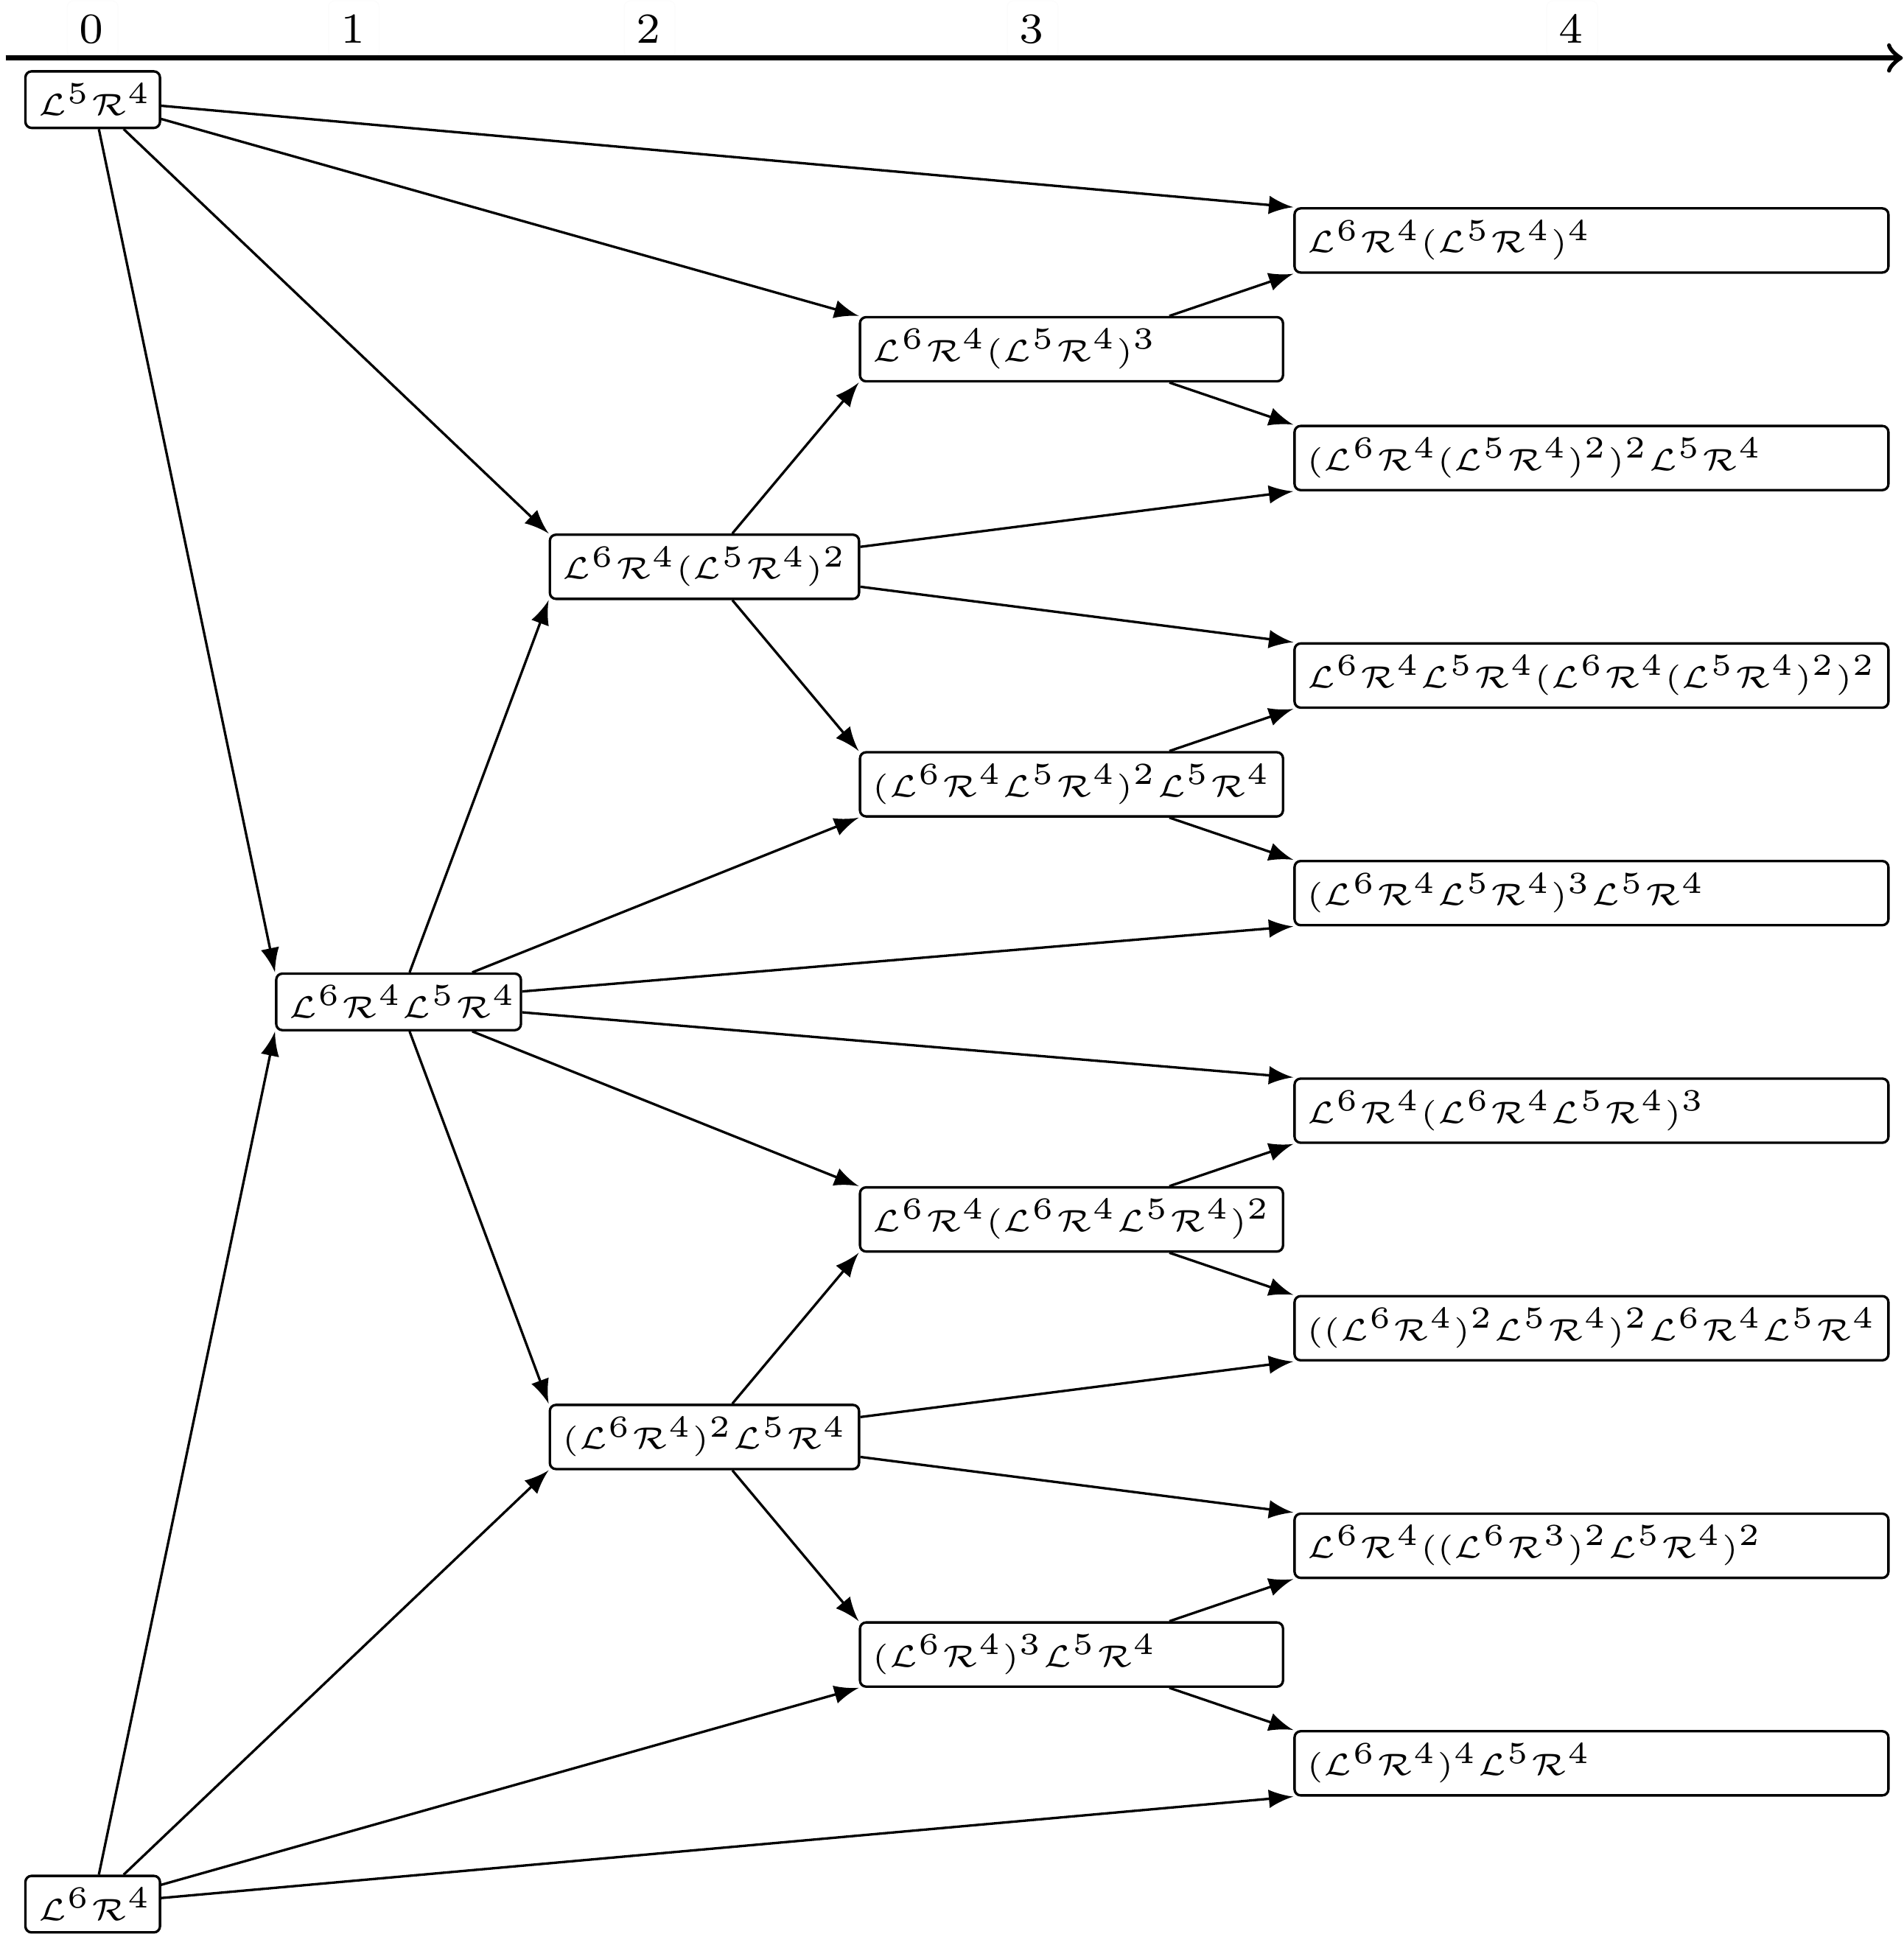
\includegraphics[width=.7 \textwidth]{FareyTrees/Minrep_Adding_larger_Halved_3/adding.png}
	\caption[Farey-tree with the symbolic sequences of a horizontal \glsentrylong{pa} structure]{
		Farey-tree with the symbolic sequences associated with the parameter regions of the horizontal \gls{pa} structure marked with a red arrow in \Cref{fig:add.halved.hor.2D} up to three levels.
		Nodes of parameter regions associated with two coexisting cycles are colored yellow.
	}
	\label{fig:halved.hor.tree}
\end{figure}

The following section will define an algorithm to translate symbolic sequences of cycles directly between the archetypal and the halved archetypal model.
This algorithm will then be used to construct rules for the periods and symbolic sequences in the \gls{pal} structures of the archetypal model.
